\subsubsection{Chaotic system under study}  \label{sec:chaos}

La familia de mapas cuadráticos bidimensionales que estudiamos aquí es modelada por un par de ecuaciones cuadráticas acopladas:
%
\begin{equation}\label{eq:mapaSprott}
 \left\{\begin{aligned}
        x_{n+1}&=a_1+a_2 x_n+a_3 x_n^2+a_4 x_n y_n+a_5 y_n+a_6 y_n^2\\
        y_{n+1}&=a_7+a_8 x_n+a_9 x_n^2+a_{10} x_n y_n+a_{11} y_n+a_{12} y_n^2
       \end{aligned}
 \right.
\end{equation}
%
donde $\{x, y\}$ son las variables de estado y $A = \{a_i, i = 1, \dots, 12 \}$ son los parámetros.
La principal característica de este sistema es que presenta múltiples atractores caóticos en función del punto seleccionado en el espacio del parámetros.
El espacio de parámetros de $12D$ generado por los coeficientes $A$ es muy difícil de explorar.

Las razones para estudiar este sistema en particular son dobles:
%
\begin{enumerate}
\item Usando la aritmética de punto flotante con un barrido automático de parámetros $a_i$ y una gran cantidad de puntos en el espacio del parámetro (alrededor de $6. 10 ^ {16}$), Sprott pudo detectar varios atractores en régimen caótico permanente.
Él también encontró una relación entre la dimensión de correlación y los exponentes de Lyapunov, con su estética visual, un tema interesante para la generación auto,ática de arte.
\item Es posible emplear estos atractores en una amplia variedad de aplicaciones electrónicas, como la generación de nuevos sistemas de encriptación, ya sea reemplazando el S-box en AES \cite{Ahmad2013, Hussain2013}, o incluso desarrollando nuevos algoritmos de encriptación \cite{Machado2004, Smaoui2009}.
\end{enumerate}

Tres de estos atractores caóticos se muestran juntos en la figura \ref{fig:atractores}.
Sus juegos de parámetros $A_i$ son:
%
\begin{align*}
A_1&=\{-0.7,-0.4,0.5,-1.0,-0.9,-0.8,0.5,0.5,0.3,0.9,-0.1,-0.9\},\nonumber\\
A_2&=\{-0.6,-0.1,1.1,0.2,-0.8,0.6,-0.7,0.7,0.7,0.3,0.6,0.9\}, \nonumber\\
A_3&=\{ -0.1,0.8,-0.7,-1.1,1.1,-0.7,-0.4,0.6,-0.6,-0.3,1.2,0.6\}.\nonumber\\
\end{align*}
%
Como se puede ver en la figura, es posible obtener salidas muy diferentes simplemente modificando el valor de los parámetros y manteniendo la estructura del sistema.
En una implementación electrónica, esto sería equivalente a poder variar la salida manteniendo la estructura del hardware y modificando los parámetros a través de, por ejemplo, una entrada.

Las figuras \ref{fig:atractores3592}.a a \ref{fig:atractores3592}.d muestran los mismos tres atractores $A_1$ a $A_3$ de la Fig. \ref{fig:atractores} junto a un atractor con $A_4=\{-1,0.9,0.4,-0.2,-0.6,-0.5,0.4,0.7,0.3,-0.5,0.7,-0.8\}$, superpuestos con sus regiones de atracción (en gris).
Las áreas blancas de cada figura corresponden a aquellas condiciones iniciales que generan trayectorias divergentes del sistema (semillas inútiles con respecto a su uso como PRNG).	
%=========================ATRACTORES 3, 5 y 9 JUNTOS =======================================
\begin{figure}
    \centering
     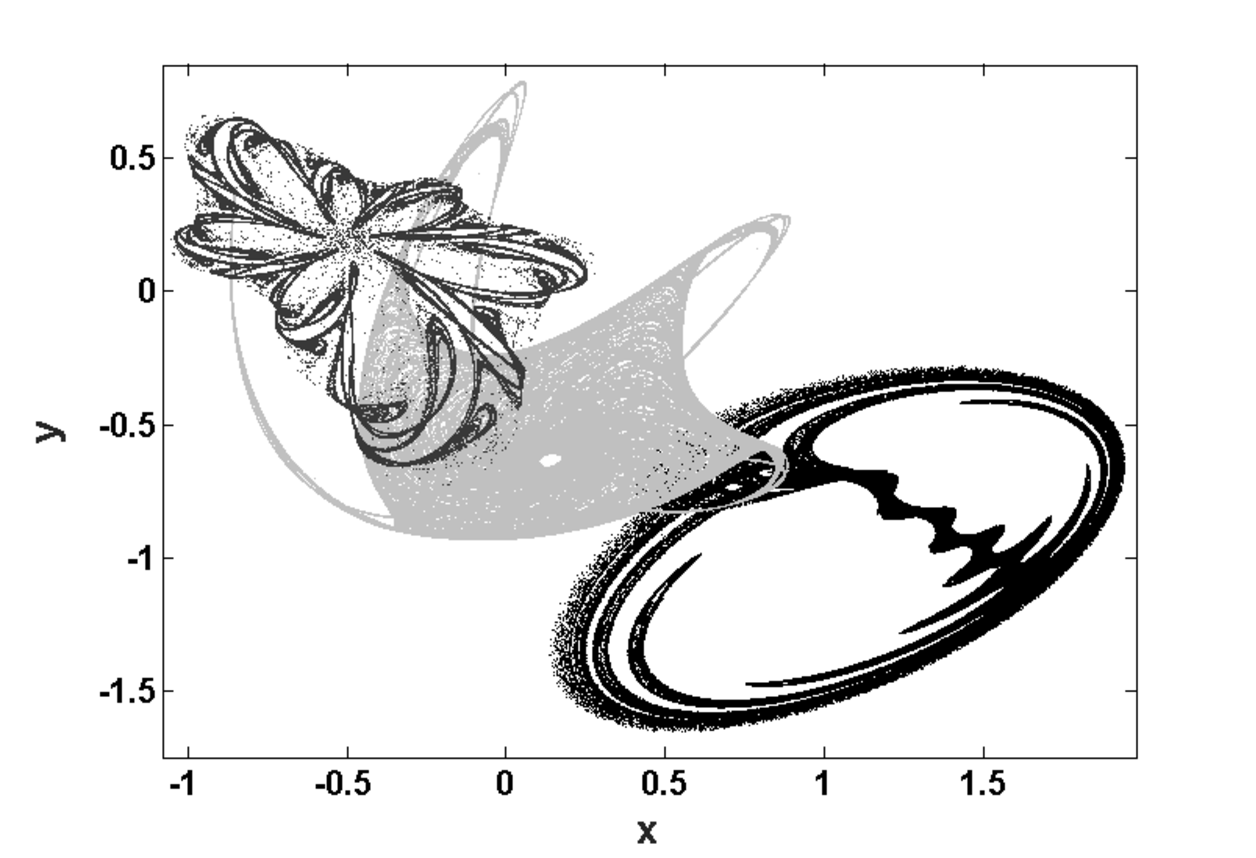
\includegraphics[width=1\columnwidth]{atractoreslindos}\\
    \caption{Tres atractores para tres juegos de parámetros distintos.}\label{fig:atractores}
\end{figure}
%====================ATRACTORES 3, 4, 5 Y 9 CON SUS REGIONES====================================
\begin{figure}
    \centering
    \begin{subfigure}[b]{0.49\textwidth}
        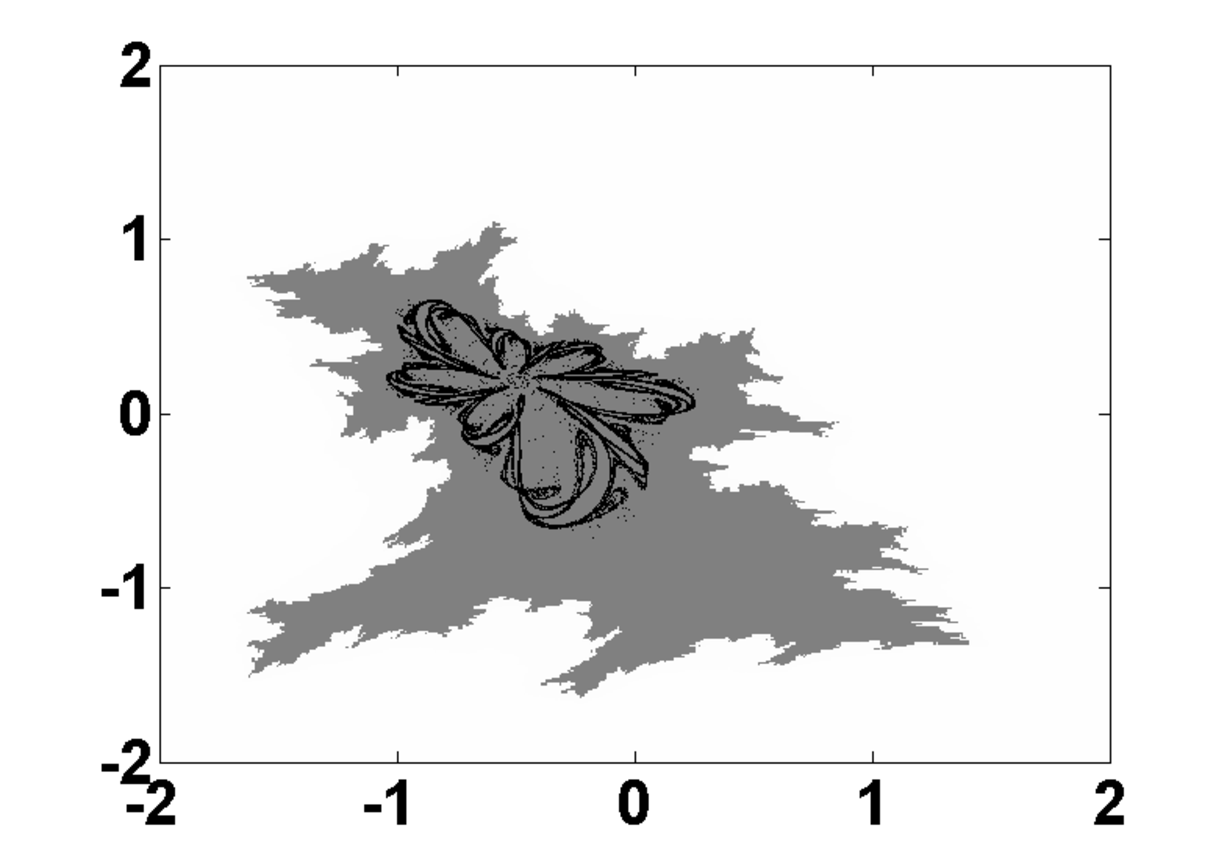
\includegraphics[width=\textwidth]{Atractor3_condominio}
        \caption{$\{a_i\}=A_1$.}
        \label{fig:gull}
    \end{subfigure}
    \hfill 
    \begin{subfigure}[b]{0.49\textwidth}
        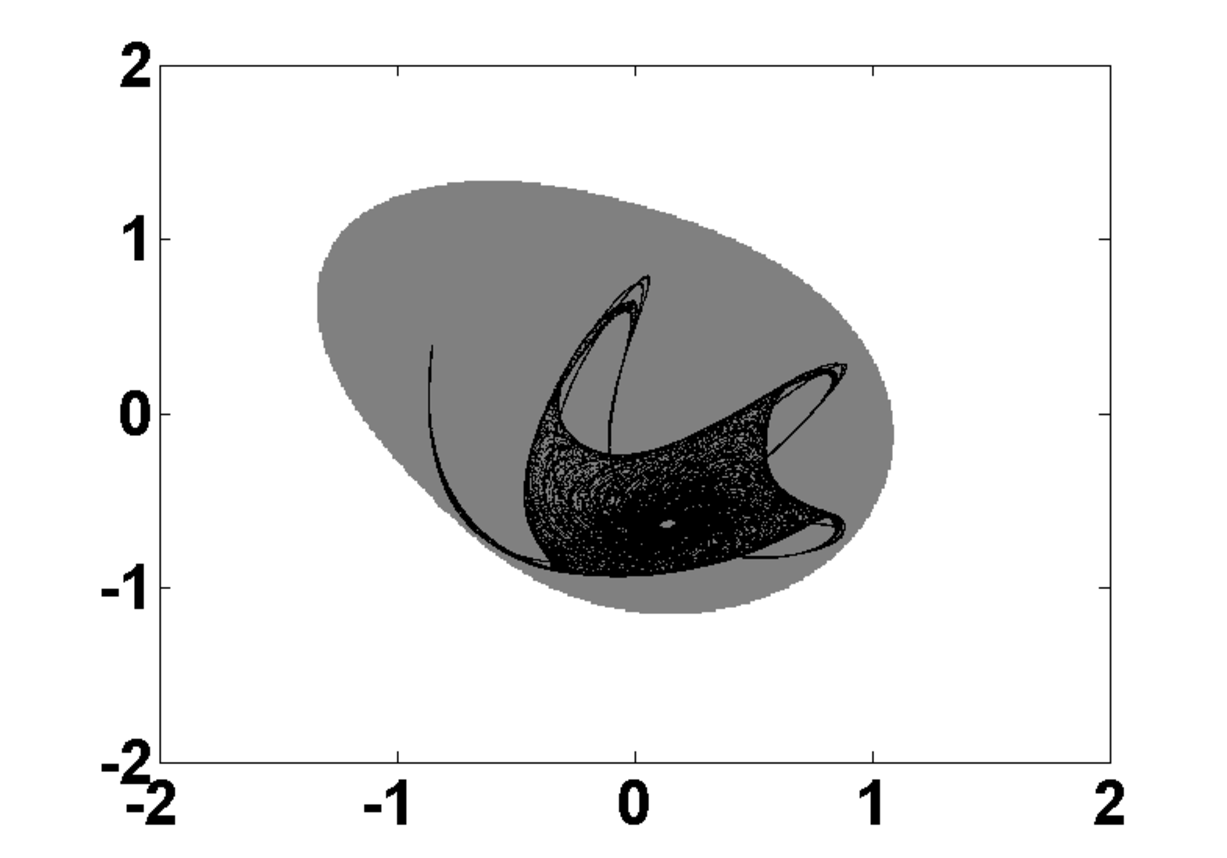
\includegraphics[width=\textwidth]{Atractor5_condminio}
        \caption{$\{a_i\}=A_2$.}
        \label{fig:tiger}
    \end{subfigure}
   \hfill 
    \begin{subfigure}[b]{0.49\textwidth}
        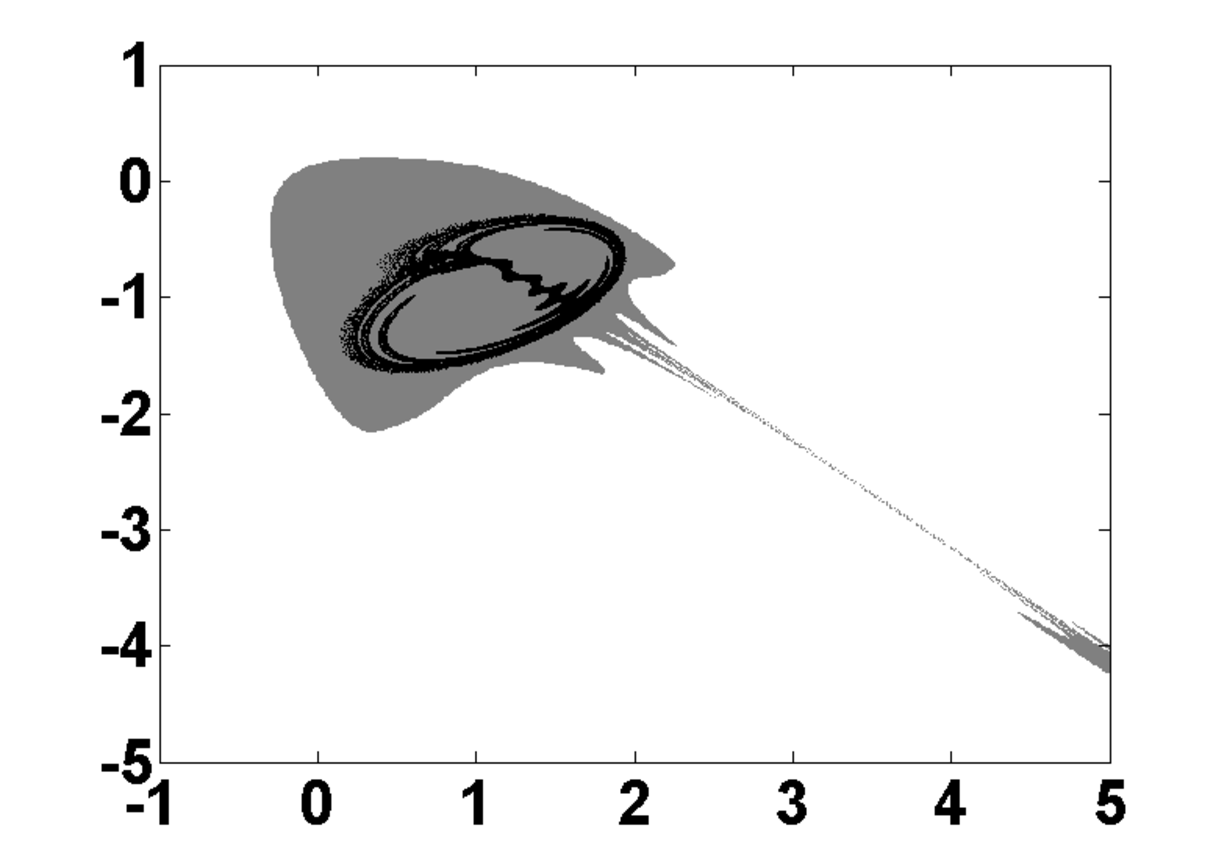
\includegraphics[width=\textwidth]{Atractor9_condominio}
        \caption{$\{a_i\}=A_3$.}
        \label{fig:mouse}
    \end{subfigure}
  \hfill  
    \begin{subfigure}[b]{0.49\textwidth}
        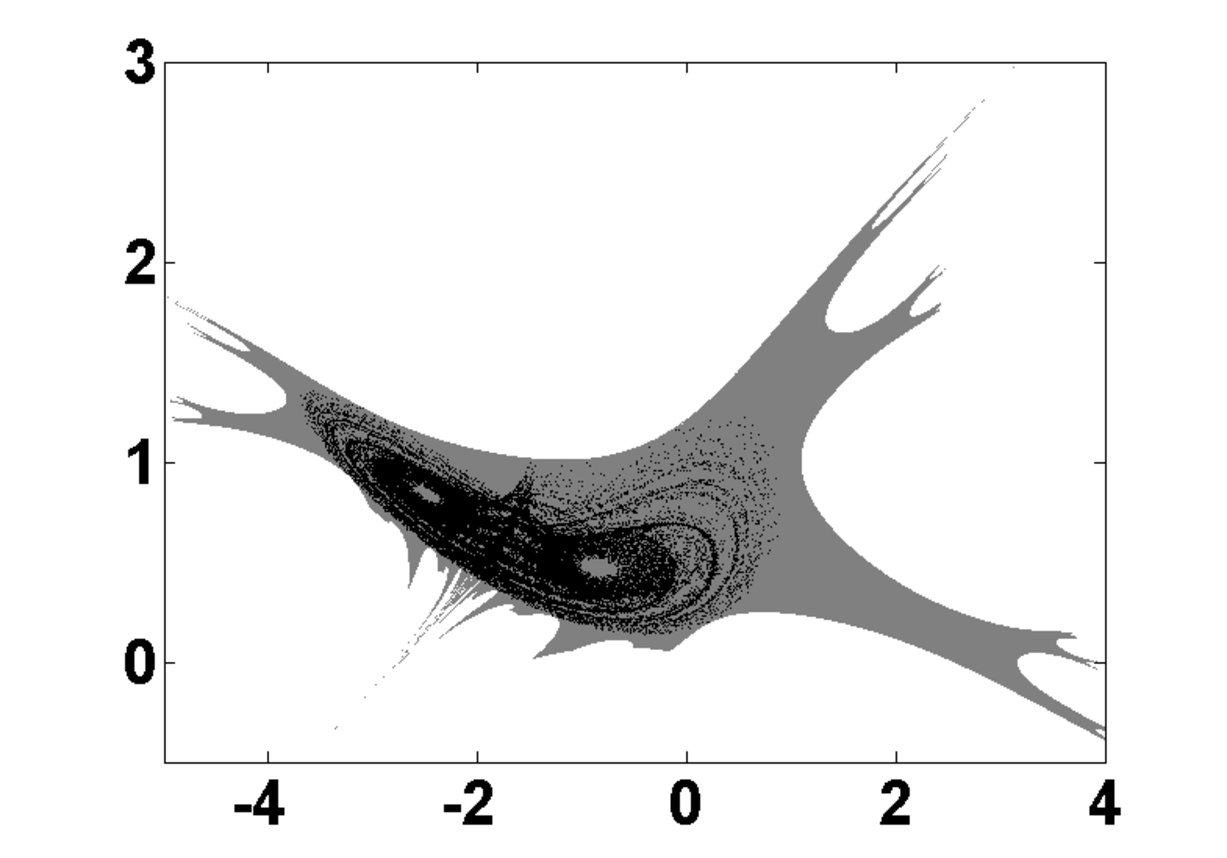
\includegraphics[width=\textwidth]{Atractor2_condominio}
        \caption{$\{a_i\}=A_4$.}
        \label{fig:mouse}
    \end{subfigure}
    \caption{Cuatro atractores caóticos y sus respectivos dominios de atracción en aritmética de punto fijo.}\label{fig:atractores3592}
\end{figure}